% File: formatting-instruction.tex
\documentclass[letterpaper]{article}
\usepackage{aaai}

\usepackage{times}
\usepackage{helvet}
\usepackage{courier}
\usepackage{graphicx}
\pdfinfo{
/Title (Temporal Planning and Inferencing for Personal Task Management with SPSE2)
/Subject (ICAPS 2011)
/Author (Andrew Dougherty)}
% The file aaai.sty is the style file for AAAI Press 
% proceedings, working notes, and technical reports.
%
\title{Temporal Planning and Inferencing for Personal Task Management with SPSE2}
\author{Andrew Dougherty\\
FRDCSA Project\\
1125 Village Center Pkwy Unit 1.  Aurora, IL 60506\\
andrewdo@frdcsa.org\\
}
\setcounter{secnumdepth}{0}

\begin{document} 
\maketitle
\begin{abstract}
\begin{quote}

SPSE2 is a free and open source software system for personal task
management that uses publicly available temporal planning systems and
tools.  It provides a GUI for users to edit planning domains
consisting of assertions about goals and their interrelations and
temporal, cost and other constraints.  It also integrates calendar and
transportation planning information.  A voice-controlled mobile
application on the Android platform for goal setting, interactive
execution monitoring and replanning is currently under development.
The rest of this paper concerns details and planned features,
application areas and future work; as well as various other AI-related
technologies being used to extend the usefulness of the core
functionality.  For example, computational semantics software will
extract models of the meaning of the goals and translate into elements
of the planning language, and deontic logics will help to determine
the consistency of the goals and plans with the user's preferred
ethics and value systems.  The work is being conducted as part of the
Cognitive Prostheses research focus of the FRDCSA project.
%% Completed

\end{quote}
\end{abstract}

\section{Introduction}

This paper documents progress within the Formalized Research Database;
Cluster, Study and Apply (FRDCSA) project towards applying existing AI
planning and scheduling tools to the domain of personal task
management.  This tool is being developed for general use, but
particularly for 1) those with disabilities impairing so-called
executive skills, and 2) those in poverty who can only secure basic
needs with difficulty.  Disabilities that affect executive skills
include Pervasive Developmental Disorders such as Autism and
Schizophrenia.  ``They are called executive skills because they help
people execute tasks.  Every person has a set of 12 executive skills
(self-restraint, working memory, emotion control, focus, task
initiation, planning/prioritization, organization, time management,
defining and achieving goals, flexibility, observation and stress
tolerance)'' \cite{cio2006}.  Additionally, the proliferation of
inexpensive Wi-Fi-enabled, Android-based smart phones, combined with
free software and perhaps solar-power chargers, has provided a novel
vector to help to supply the homeless or similarly disadvantaged with
practical, survival-oriented computing resources.  Anecdotal evidence
suggests further that the executive skills of those even without such
limiting factors still may have room for improvement, especially when
compared to a more optimal automated negotiation and coordination of
temporal constraints and privacy preferences.  Such improvements in
local planning efficacy and resource utilization could have
macroscopic effects and relax otherwise exacerbated resource
conflicts.  Additionally, the application of user-defined ethical
analytics through computational deontology offers a method to
constrain the space of possible actions that are available to
intelligent personal agents.  Therefore, development of a free and
open source (FOSS) personal task management system that interfaces
with existing sources of data such as calendars, routing applications
and mobile phones promises to help to improve the quality of life
generally.
%% Completed

\subsection{Overview of the FRDCSA Project}

\noindent The first and major goal of the FRDCSA project, 11 years and
running, is to help to provide for better security and quality of life
for all sentient beings.  A major assumption is that FOSS artificial
intelligence, engineered correctly and with unlimited redistribution,
satisfices this goal.  To avoid polemics, the project is concerned
only with implementing a restricted form of weak AI.  The approach,
motivated by algorithmic information theory and information-theoretic
computational complexity of metamathematics
\cite{Chaitin74information-theoreticlimitations}, has two prongs - to
develop an increasingly complete theorem proving system and library
(called Formalized Research Database (FRD)), and to develop an
increasingly complete collection of practical software (Cluster, Study
and Apply (CSA)).  Perhaps, the two approaches are in some sense
theoretically equivalent by the Curry-Howard isomorphism, which would
seem to say that the classes of programs and proofs are coextensive.
So ideally the FRD is a practical, transfinite implementation of
Hilbert's program, which can never be completed, but which can, by
engineering a sequence of logics each more complete than the previous,
decide in the limit all problems that are not absolutely undecidable
(should any of those exist).  This idea may be similar to or the same
as one of Turing of creating a sequence of logics, each more complete
than the previous, based upon the assumption of the existence of
increasingly large constructible ordinals \cite{turing1939}.
Alternatively, the CSA consists of a set of programs for building and
packaging most or all known freely available software systems and
datasets.
%% Completed

The primary goal of the project and limitations to personal
productivity necessitate the development of tools, including a
personal task management system, which provide tangible benefits to
all users and in particular those working on FOSS software
development.  Yet such a system has been reasonably difficult to
engineer in the context of the project, as evidenced by the almost 10
such systems in various stages of completion, many not mentioned here.
Also, it has been difficult to find an accurate name for this entire
collection of functionality.
%% Completed

\subsection{Overview of the SPSE2 System}

\noindent SPSE2 is a system for personal task management.  It provides
a GUI for users to edit planning domains.  These domains consist of
assertions in a knowledge base regarding goals, their interrelations,
and constraints of types such as temporal and cost.  This GUI allows
users to specify the constraints, and then the domain is converted
into a PDDL domain and a plan generated.  Future versions will include
a fully functional and re-engineered interactive execution monitor
that will walk the users through the plans and allow replanning from
hands-free, voice-controlled cell phones.  Ideally the interface would
expand to handle more types of plans besides linear.  There are
several primary FRDCSA systems involved architecturally, including the
Universal Language (UniLang), Free Knowledge-Based System v2
(FreeKBS2), Verber, and Planning, Scheduling and Execution (PSE)
systems.

\begin{figure}[h!]
  \centering
      \includegraphics[width=84mm]{images/ps/spse2.ps}
  \caption{Shared Priority System Editor v2}
\end{figure}

%% Completed

\section{System Architecture}

\subsection{Shared Priority System Editor}

The name SPSE2 derives from Justin Coslor's concept of Priority
Systems \cite{coslor2008}.  Our goal system is straightforward, it has
goals as nodes, unary predicates as conditions, and binary predicates
as edges.  Here is related metadata from a sample goal in a planning
domain.  Suppose {\tt <REL>} is {\tt ("entry-fn" "pse" "38")}:

\begin{footnotesize}
\begin{verbatim}
("asserter" <REL> "unknown")
("goal" <REL>)
("has-NL" <REL> "ICAPS 2011 Paper")
("has-source" <REL>
 ("entry-fn" "sayer-index" "806"))
("depends" <REL> ("entry-fn" "pse" "17"))
...
\end{verbatim}
\end{footnotesize}

\noindent Goals are straightforwardly expressed in natural language,
and may be marked with a unary predicate (such as {\bf complete}, {\bf
  showstopper}, {\bf deleted}, {\bf cancelled}, {\bf ridiculous}, {\bf
  obsoleted}, {\bf rejected}, and {\bf skipped}), or by a binary
predicate (such as {\bf depends}, {\bf provides}, {\bf eases} and {\bf
  prefer}).  SPSE2 is used to develop the planning domain, stored in a
FreeKBS2 context (equivalent more or less to CYC's microtheories).
The SPSE2 planning domain is converted to a domain usable by Verber,
which then generates a PDDL domain.  Implementation of more complex
models of the semantics of processes is postponed until the basic
system is completed.  Eventually, goals that are ongoing or recurrent
(i.e. do the laundry) should be modeled.  For now, it only concerns
whether a given goal has been completed.  The SPSE2 GUI is being
extended to become a knowledge editor, by adding several additional
often related node types and predicate sets and background knowledge.
There is also a domain for general knowledge modeling.  The GUI has
special functions for each domain.  Domains under development
include:\\

\noindent {\it Alethic, Argumentation, CLEAR, Contexts, Critic, Deontic, Discourse\-Representation, Doxastic, Genealogy, Intelligent\-Agent, Intelligent\-Tutoring, Inventory, Metamathematics, Network\-Mapper, PIC\-Form, Planning, POSI, Social\-Networking, Suppositional\-Reasoner, Tactics, Temporal, Workflow}\\
%% Completed

\subsection{FreeKBS2}

Knowledge is stored in FreeKBS2.  FreeKBS2 can convert between several
notations (KIF, Emacs and Perl Interlingua, CycL, etc) and will
eventually have more back-ends besides the current Vampire-KIF
back-end, enabling reasoning over higher-order and modal logics.
Vampire provides first-order theorem proving with equality.
%% Completed

\subsection{Verber}

In order to generate a plan, SPSE2 translates its domain into one
usable by Verber.  Verber, named after the late Senior Chess Master
Richard Verber, is basically a wrapper around various PDDL planners.
Verber provides a set of Perl modules for building and interacting
with PDDL domains (and hopefully other planning formalisms eventually)
for calling various planners and parsing the results.  It also houses
a primitive knowledge engineering aspect for constructing Verb format
planning domain libraries tailored to the specific domains required in
the project, such as movement discipline, goal tracking and meal
planning.  The Verb format is a very lightly extended PDDL, which
allows importing other domains and problems and also a way to convert
between PDDL's scalar time values and actual dates and times.  Ideally
Verber is capable of observation, learning the average and worst case
durations of certain types of actions or events, and incorporating
this into the plan development.  Currently, there are several planners
that are partially integrated, but so far LPG-TD is used primarily
\cite{gerevini2004}.
%% Completed

\subsection{UniLang}

\noindent The UniLang system is an interprocess communication system
for Perl ``agents''.  UniLang is loosely termed a multiagent system,
patterned off of the Open Agent Architecture, but without most of the
Prolog-based communication capabilities (although it does have a
trivial FreeKBS2-based knowledge interchange capability).  Most
agents, such as FreeKBS2, Verber and SPSE2 main and temporary agents,
communicate with each other through the {\bf Send} or {\bf
  Query\-Agent} functions.
%% Completed

\subsection{PSE}

\noindent PSE stands for Planning, Scheduling and Execution.  It is
one of the older FRDCSA planning systems.  While the original design
using object-oriented Perl code has been replaced entirely with the
PDDL-based approach through Verber, there remains a significant
collection of Emacs Lisp code within the namespace that works with the
new Verber model.  Before SPSE2, Emacs was the primary way of
interacting with the planning system.  Several interfaces were
developed for manipulation of goals.  Significant to note are the
functions for rapidly asserting relations between goals.  A
stack-based interface, similar to an RPN scientific calculator, exists
for pushing textual entities under the Emacs point onto the current
stack, operating on the contents of the current stack and ring of
stacks, and asserting into FreeKBS2.  One such function will return
the entry ID of the goal corresponding to the text under the Emacs
point.  This interface is still very much under development for the
Natural Language Understanding (NLU) system and the Knowledge-Max
editor (KMax) systems, allowing semantic markup of text and consequent
rapid manipulation of symbolic, textual knowledge.
%% Completed

\section{System Interfaces}

\subsection{Calendar Synchronization}

In order to improve the utility of Verber, a calendar synchronization
feature has been developed.  This allows synchronization with ICS
Calendars or Google Calendars, the ICS files for which are obtained
and then translated into the SPSE2 domain representation.  In order to
schedule an event occurring at a certain time, it is translated from
the date and time information into the offset and scale of the scalar
planning time value.  The event start date is marked using PDDL timed
initial literals.

\begin{footnotesize}
\begin{verbatim}
(at 1.00 (possible <EVENT>))
(at 2.00 (not (possible <EVENT>)))
\end{verbatim}
\end{footnotesize}

\noindent Additionally the planning domain includes the following
precondition for the durative action {\bf Complete}.

\begin{footnotesize}
\begin{verbatim}
(over all
 (or
  (not (has-time-constraints ?e1))
  (possible ?e1)))
\end{verbatim}
\end{footnotesize}

\noindent Here is an example of the time constraints that are asserted
by the DateTime interface.

\begin{footnotesize}
\begin{verbatim}
("end-date"
 ("entry-fn" "pse" "38")
 "TZID=America/Chicago:20101129T120000")
\end{verbatim}
\end{footnotesize}
%% Completed

\subsection{Notification Manager}

\noindent A Perl/Tk-based notification manager patterned off of the
Android notification manager has been completed partially.  Ideally,
it would be able to synchronize with the Android notification manager.
Certain tasks that regularly occur are regularly added to the SPSE2
planning context by a cron job.  The custom cron-like format includes
information on how much warning time should predate the beginning of
the possibility of completing a task.

\begin{figure}[h!]
  \centering
  \includegraphics[width=84mm]{images/ps/notification-manager.ps}
  \caption{Notification Manager}
\end{figure}

%% Completed

\subsection{Deontic and Teleologic Logics}

\noindent It should be possible for users to place certain ethical
constraints on possible actions, in order to provide their agents with
a moral decision support system.  In support of this, work is ongoing
to formalize various systems of morality in terms of deontic logics,
and to provide an evaluation function which evaluates individual
actions and plans against various selected moral systems.  Therefore,
the user simply declares the moral systems to which they agree, and
the system then evaluates the actions.  To illustrate a glaring but
simple example, let us consider the Ten Commandments, specifically the
obligation that ``Thou shalt not kill''.  If our computational
semantics lacked understanding of general prohibitions, perhaps this
could be manually translated to ``Someone or something murdered''.
This is then converted to a logic form {\tt <LF>} and it asserts:

\begin{footnotesize}
\begin{verbatim}
(implies <LF> (rule-activated <RULE-NUMBER>))
\end{verbatim}
\end{footnotesize}

\noindent It then determines whether this rule is activated using
semantic textual entailment recognition.  The recognizer would load
the logic of the plan and all enumerable consequences, convert to
logic form, instantiate the variables with their valuations, add
contingent background knowledge, and query: {\tt (rule-activated ?X)},
relaxing the lexical constraints until a rule is activated.  Of
course, in practice this will be more complicated
\cite{Balduccini06knowledgerepresentation}. Besides considering
general obligations and prohibitions (deontics), it should also be
useful to consider a means-ends analysis (teleologics).
%% Completed

\subsection{World State Comparison and Value Systems}

\noindent An intended capability is to enable reasoning intelligently
about the value of a given plan or outcome.  In trying to evaluate
various actions to determine which are morally superior according to
various moral theories, it begs the question of which world-states and
histories are preferable.  To evaluate this, a general comparison
function needs to be developed.  To reduce the evaluation to a total
order would be somewhat dualistic - but ultimately the user should be
able to choose preferable from among possible worlds - or rather
provide rules which in some sense order them.
%% Completed

\subsection{Android Bluetooth Headset-Based Interactive Execution Monitor}

\noindent In order to provide a usable interface to the plans, an
application for the Google Android mobile operating system is being
developed for recording new goals, walking the user through generated
plans, and initiating replanning.  Currently, a client-server system
has been implemented that communicates between the phone and server
using XMLRPC.  This functionality actually resides within UniLang.  A
limited set of voice commands has been developed, enabling the phone
to for instance answer factoid-based questions using our agent
wrapping the open source OpenEphyra question answering system.  Here
is an illustrated use case for this kind of question answering.  The
user initiates the speech interface by pressing a certain combination
of buttons on their Bluetooth headset, currently only the media button.
Recognition occurs using Google's voice recognition API, and results
are then sent via XMLRPC to the Android-FRDCSA-Server UniLang agent.
The command is processed by a VoiceCommand module, which in this use
case sends a query to the QUAC Question Answering system, before
ultimately returning the message.
%% Completed

Previously, a text-based interactive execution monitor was deployed
which used the Sphinx2 numeric domain and TTS to query the user as to
the status of the completed plan.  Thus, it is not hard to imagine
adapting the current text-based interactive execution manager to work
on the Android phone.  Progress was delayed for months while the
development phone was broken, but thankfully another unit has been
procured recently.  Initiating communication to the phone, on the
other hand, while more difficult, may be accomplished either through
registering the phone with a dynamic-DNS provider, or by polling from
the phone to the server.  Voice commands for controlling the process
of planning, replanning and the interactive execution monitor will be
developed.  Development of the interactive execution monitor,
especially one that incorporates conditional planning for various
possible interaction situations (such as whether the user is in the
presence of the phone or the computer), will be more difficult.
%% Completed

\subsection{Location Logic}

\noindent Location Logic is a system for inferencing with the
semantics of logic related to the users' physical locations as
reported by the GPS (or in the multiagent case using location services
like Google Latitude), as contrasted to their waypoint data.  It works
by asserting theorems observed regarding the GPS tracks, such as
whether certain waypoints are being approached, visited, or departed.
Location Logic interfaces naturally with the SPSE2 system.  Locational
restrictions will be extracted from goals using named entity
recognition and computational semantics.  Eventually, multiagent,
distributed planning solvers should be integrated which are able to
resolve distributed resource problems.

\begin{figure}[h!]
  \centering
  \includegraphics[width=84mm]{images/ps/location-logic.ps}
  \caption{Location Logic Prototype}
\end{figure}

\noindent Here is an example use case.  Suppose both Alice and Bob are
using mobile phones having the hands-free voice-controlled task list
and Location Logic systems installed.  Both Alice and Bob are wearing
Bluetooth headsets.
%% Completed

So suppose Alice is out of milk, but she doesn't know this right away.
(Perhaps her roommate drank the last of it, and did not or could not
tell her yet).  Meanwhile, Bob is out running errands of his own.
Alice wakes up and comes down the stairs and goes to get some cereal.
She pours the bowl of cereal and then looks in her refrigerator.  She
realizes that the milk is empty and has not been thrown out.
Disappointed, she taps a button on her Bluetooth headset.  It responds
``Yes?''.  Alice says: ``pantry remove item milk'', to which her
headset responds, ``Confirm remove milk from pantry inventory?''.
Alice says ``yes'' and the headset responds ``Milk removed''.
%% Completed

When Alice tells the system that she was out of milk - the system
realizes according to various considerations that she should buy some
more milk.  It therefore automatically added the goal ``get milk''.
Because Alice and Bob are friends, they have already told their Shared
Priority Systems that they can collaborate on several matters, one of
which is food inventory.  Perhaps Alice's planning agent sent a
broadcast to all of her friends with which she shares this particular
kind of information.  It was stated simply as the goal that there
should be a fresh jug of milk in Alice's refrigerator.  The various
agents therefore add this goal to their own planning systems.
Collectively, at the next planning or replanning cycle, using a
distributed planning formalism, they agree on the details of the least
costly and most preferable plan that incorporates Alice's request.
Bob's planning agent and ethical analyzer agree to propose to Bob the
task of picking up and dropping off milk to Alice's house, because he
was approaching a grocery store, didn't have other things that
couldn't be slightly postponed, and his adjustable autonomy settings
allowed for the proposal.  Bob and perhaps Alice get a message
suggesting that this action be taken.  Once both have agreed, it is
added to the planning system, even including so much as to tell Bob's
cell phone agent which type of milk Alice would like.  Bob then
purchases the milk and then swings by Alice's place on his way to
work.  For now, assume Alice pays him cash - but in the future an
automated distributed loan/payment system will be used.
%% Completed

The usefulness of the milk provision scenario is debatable, but
certainly in the general case such efficient team-based collaboration
would be very desirable, as for instance in the case of ride-sharing,
shared task management, and so on.

Here is an example Location Logic rule.

\begin{footnotesize}
\begin{verbatim}
(implies
 (and
  (leaving ?AGENT ?LOCATION)
  (isa ?LOCATION movie-theatre)
  (has-performed-action ?AGENT
   "silence cell phone at movie theatres")
  ;; (> (sitting-still) (minute 1))
  )
 (perform-action "add-to-pending-tasks"
  "unsilence cell phone \
   when leaving movie theatres"))
\end{verbatim}
\end{footnotesize}

\subsection{Federated Transportation Planning}

\noindent A federated transportation planning option, based on the
FRDCSA BusRoute planner
\footnote{http://frdcsa.org/frdcsa/internal/busroute} has been
integrated with Verber.  However, with the advent of Google's public
transportation planner it will be replaced.  This interface should
naturally understand waypoints, and be able to generate queries to a
public or private transportation routing system in order to populate
the planning domain with the timing constraints.  Ideally services
transmitting actual bus positions and timing could be integrated - and
replanning initiated as needed.
%% Completed

\section{Systems Using SPSE2/Verber/PSE}

\subsection{POSI Collaboration}

\noindent The planning system and interactive execution monitor have
several applications.  One related project using the tools of the
FRDCSA is the POSI Open Source Initiative (POSI)
\footnote{http://intranet.posi.frdcsa.org}. It is a project for
representing the goals, interests and abilities of its users, as
distilled from their writings and volunteered information.  The idea
is to establish necessary and sufficient information to form dynamic
multiagent teams to solve problems that are shared between multiple
persons.  Priority Systems are essentially networks of goals and
constraints on these goals.  Future versions of SPSE will be able to
simultaneously edit the same Shared Priority Systems.  Various models
of shared editing are under consideration.  Ideally, when someone
marks a goal as completed, the other SPSE agents should display such
changes.  An analogy can be made to a real-time strategy game.  An
essential feature of POSI is identifying when different users have
specified the same or related goals.  This is accomplished chiefly
using the nascent technology of Textual Entailment Recognition, as
well as through breaking down individual goals into more clearly
defined or achievable steps.  As such, the Goals, Interests and
Abilities (GIAs) of the users are modeled using ontological tools.
SPSE2 itself soon will have the ability to edit domains besides
temporal planning, including different ontologies such as the POSI
ontologies.
%% Completed

\subsection{Akahige Medical System}
Another intended application is the Akahige Medical System
\footnote{http://frdcsa.org/frdcsa/internal/akahige}.  One capability
of the Android phone-based general purpose help system under
development is to launch a medical help system in the event that any
conspicuous symptoms occur or at regularly scheduled times.  Symptoms
may be run through a standard or custom medical diagnostic program
(such as Diagnosaurus or the planned Akahige Model-Based Diagnostic
and Fault Localization software).  The result of the diagnostic
procedure may require an emergency response.  In such a case,
instructions for the given emergency or situation will exist within
the system and the user will be guided by the interactive execution
monitor to complete these tasks, and to refer to documentation as
needed.
%% Completed

\subsection{Gourmet Meal Planner}

Another area of significant interest is meal planning.  The FRDCSA
project includes a meal planner, called Gourmet
\footnote{http://frdcsa.org/frdcsa/internal/gourmet}. It will
interface with our inventory management component for pantry
management.  The SOAR archive of around 150,000 meal-master recipes is
being integrated.  Work is progressing on developing a foodstuffs
ontology, upon which to map the ingredients and intermediate
foodstuffs of recipes.  Mapping to nutrient databases such as the SR23
and also to product databases such as UPCdatabase.com, in addition to
formalizing the recipe steps into discrete planning operations, will
provide all the resources required to achieve interactive recipe
execution through the Android interface.  The formalization of recipe
steps will hopefully be attempted by training CMU's StackedFrameParser
on the CURD/MILK dataset of annotated recipes.  They use a medium
grained language called CURD which expresses a set of abstracted
operations on food and intermediate foodstuffs \cite{tasse2008}.  Then
arbitrary English recipes may be attempted.  As some other open source
meal planners have well established user bases, this automatic
annotation could be performed and cached by a web server (as the
StackedFrameParser requires 8GB of RAM), and could be augmented and
trained by user corrections given a sufficient GUI and upload
mechanism.
%% Completed

\subsection{Paperless-Office System}

Another FRDCSA project that will make use of the planning technology
is the
Paperless-Office \footnote{http://freshmeat.net/paperless-office}.
With this system, which already functions to scan, OCR, search and
edit documents, it will be possible to specify workflows - such as
certain documents requiring to be filled out and sent by certain
times.

\begin{figure}[h!]
  \centering
      \includegraphics[width=84mm]{images/ps/paperless-office.ps}
  \caption{Paperless-Office}
\end{figure}

%% Completed

\subsection{SystemX Intelligent Tutoring System}

Work has been ongoing on Arbitrary Document Understanding.  Being able
to represent the argument structure of a text, and also the facts and
relations of the text, enables the generation of temporal plans for
teaching subjects at various granularities based on various learning
objectives and timing constraints.  A prototype system called Study
has been developed \footnote{http://frdcsa.org/frdcsa/internal/study}.
SystemX will use the SPSE2 or its derivatives.
%% Completed

%% \subsection{Story Understanding and Generation}

%% An area of interest is in story understanding and generation (not to
%% mention poetry).  So for instance, the exposition structure of this
%% LaTeX paper was modelled using a planning domain, although specialized
%% domains are/will be developed.  These domains necessarily use the
%% various other the domains, such as multiagent modeling capabilities,
%% of SPSE2 - to model what the authors intended effects are on the
%% audience and to generate stories that match these goals.  Currently,
%% Ryan McGregor and I are working on a video game called ``The Revival''
%% which incorporates story generation and multiagent simulation using
%% the FRDCSA.
%% %% Completed

\section{Conclusions and Future Work}

\noindent Usable Perl/Tk, Emacs and Android systems for editing goals,
adding temporal constraints, generating plans, and walking the user
through them are close to completion.  The chief obstacle to the
release of this work has been its thorough dependence on the FRDCSA, a
large set of heavily interconnected yet unreleased software.  A proper
requirements engineer process should be initiated (as the project
management for SPSE2 is currently performed within SPSE2 itself - a
chicken and egg problem).  The completion of the Android interactive
execution monitor is now possible following the recent acquisition of
a working Android phone.  As well, some pernicious bugs affect the
FRDCSA notification manager.
%% Completed

There are several other related topics that bear mentioning but that
unfortunately time constraints have precluded.  This includes plan
libraries (including some other previously developed PDDL domains for
personal tasks involving several other predicates), ontological
modeling, scripts and automatic execution of tasks, house rules,
textual entailment, computational semantics via logic forms, static
domain analysis, reasoning with the consequences of failing to
complete certain tasks, automated goal analysis, an ontology of
planning systems and their capabilities, plan cycles, and
incorporating conformant and other plan types into the interactive
execution monitor.  Here are some important areas for future work.

\subsection{Automatic PDDL Domain Construction Via Computational Semantics}

\noindent Although currently goals are simply evaluated in a boolean
context, a more detailed interpretation of the semantics of the goals
is planned.  Ideally, it would convert the natural language contents
of goals and other node types into a logical semantic representation,
such as logic forms (LFs), and from the LFs construct the PDDL domains
and problems.
%% Completed

\subsection{Suppositional Reasoner}

\noindent The suppositional reasoner seeks to incorporate more
positional evaluation and analysis of domain invariants, domain
specific knowledge and so on, into the planning process.  It ideally
would function as a plan development and critiquing interface for
real-life problems, hopefully allowing the evaluation of any decision
making process.  It is being calibrated on domains like Chess and Go
that have a substantial literature that may be formalized and in which
feedback on efficacy is relatively short.  From a search point of
view, it is not very interesting, for starters some standard search
algorithms should be implemented.  But attempting to hybridize the
search with positional information is interesting.  Annotated chess
games and their logic-based formalizations are being used to develop
knowledge that may be tested and applied to the situation.  The Sayer
system provides a method for a kind of theorem proving over these
domains and to perform Natural Language Understanding (NLU) within the
project.

%% Completed

\subsection{Temporal Conformant Planning}

One desired capability is temporal conformant planning, and tools for
exploring the set of actions possible to the agent at each state, and
reasoning with the consequences of various choices at that point.
This naturally reflects back to the suppositional reasoner and the
valuation system.  This is perhaps related to Conditional Temporal
Planning \cite{Tsamardinos03ctp:a}.  Tools that implement these
techniques should be located and integrated.
%% Completed

%% Basic functionality in lieu of temporal conformant planners is to fork
%% domain at each environmental decision point and generate plan - store
%% plan hierarchy, also which nodes have no plan and require domain
%% re-engineering

\section{Acknowledgments}

\noindent I am grateful especially to Aloysius Flori and my immediate
family who have been supportive of my work; to Justin Coslor who has
provided the inspiration for countless systems and programs and has
developed a formal theory of context; to the CMU community for its
helpfulness; to Jim Oberweis and the late Richard Verber for their
support and mentorship with chess; and to the many persons who showed
me kindnesses when they were under no obligation to do so.
%% Completed

I wish to thank all of the researchers who have or will have provided
references and pointers, those who have made progress in this field,
and in particular those who have released software, documentation and
papers under freely redistributable or preferably FOSS licenses, such
as the authors of LPG-TD. Such licenses make the work of an open
source systems integrator much easier.
%% Completed

\bibliographystyle{aaai} \bibliography{icaps-2011-paper}

\end{document}
